\documentclass[letterpaper, 12pt]{article}
\usepackage{graphicx} % Required for inserting images
\usepackage{textcomp}
\usepackage{fullpage}
\usepackage{amsmath}
\usepackage{xcolor}
\usepackage{float}
\usepackage{geometry}
\usepackage{biblatex}
\geometry{margin=1in}
\usepackage{enumitem}
\usepackage{microtype}
\usepackage{gensymb}
\usepackage{parskip}
\usepackage{tikz}
\usepackage{caption}
\usepackage{cancel}
\usepackage{nicefrac}


\usepackage{hyperref}
\hypersetup{
    colorlinks=true,        % Enable colored links
    linkcolor=teal,         % Set color for internal links
    citecolor=teal,         % Set color for citations
    filecolor=teal,         % Set color for file links
    urlcolor=teal           % Set color for URLs
}

\usepackage[version=4]{mhchem}

\title{Practice questions and explanations}
\author{BIOS 1006}
\date{Week 1}

\begin{document}

\maketitle

\section*{Lecture 1: Fundamentals}

\subsection*{Functional groups}

\subsubsection*{Question 1: Naming}

\begin{figure}[H]
\centering
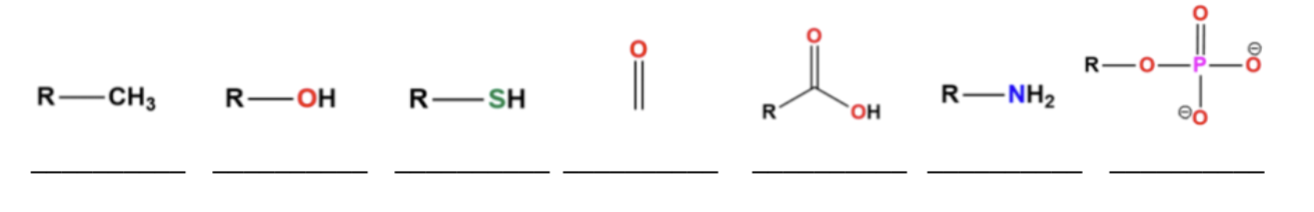
\includegraphics[width=0.9\textwidth]{functionalgroups}
\end{figure}

Answers:

\fbox{methyl, hydroxyl, thiol, carbonyl, carboxyl, amino, phosphate}

\subsubsection*{Question 2: Roles of functional groups}

\begin{enumerate}
\item Amino acids and proteins have \fbox{amine} groups \& \fbox{carboxyl} groups.
\item Carbohydrates tend to have an abundance of \fbox{hydroxyl} groups and \fbox{glycosidic} linkages.
\item Lipids vary greatly in structure, but fatty acids typically have \fbox{carboxyl} groups.
\item Each nucleotide in a nucleic acid molecule has \fbox{phosphodiester} linkages.
\end{enumerate}

\subsection*{pH and pKa}

\subsubsection*{Question 3: ICE tables}

You make a 0.2 M aqueous solution of propionic acid \ce{CH3CH2COOH} by dissolving an appropriate amount of propionic acid in water. The pH of the resulting solution is 4.88. What is the Ka of propionic acid?

$$\ce{CH3COOH \rightleftharpoons CH3COO- + H+}$$

Set up the ICE table:

\begin{table}[H]
\centering
\begin{tabular}{c|c|c|c}
& \ce{CH3COOH} & \ce{CH3COO-} & \ce{H+} \\\hline
Initial & 0.2 & O & O \\
Change & -x & +x & +x \\
End & 0.2-x & +x & +x \\
\end{tabular}
\end{table}

\section*{Lecture 2: Amino acids and peptides}

\subsubsection*{Question 4: Amino acid chemical properties}

\paragraph{Which amino acid side chains are ionizable?} YECDHKR

\paragraph{Which amino acid has no chiral center?} G

\paragraph{Which amino acids have hydrophobic (nonpolar) side chains?} AVLIGMPFWY

\paragraph{Which amino acid side chain has an amino group?} K

\paragraph{Which amino acids have basic functional groups?} RHK

\subsection*{pI of a peptide}

\end{document}